\documentclass[tikz,border=8pt]{standalone}
\usepackage{amsmath,amssymb}
\usetikzlibrary{arrows.meta,calc}
\definecolor{TargetBlue}{HTML}{2364AA}
\definecolor{NuisanceOrange}{HTML}{E6862A}
\definecolor{EfficientGreen}{HTML}{278A64}
\definecolor{NeutralGray}{HTML}{68717C}
\begin{document}
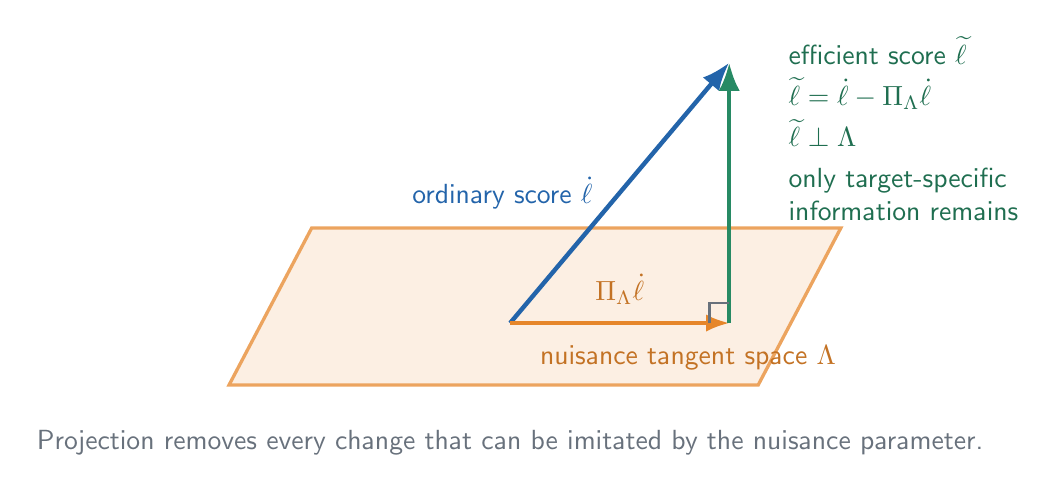
\begin{tikzpicture}[font=\sffamily, >=Latex, scale=1.05]
  \fill[NuisanceOrange!13] (-3.4,-0.75) -- (3.0,-0.75) -- (4.0,1.15) -- (-2.4,1.15) -- cycle;
  \draw[NuisanceOrange!75, very thick] (-3.4,-0.75) -- (3.0,-0.75) -- (4.0,1.15) -- (-2.4,1.15) -- cycle;
  \node[text=NuisanceOrange!85!black] at (2.15,-0.42) {nuisance tangent space $\Lambda$};

  \coordinate (O) at (0,0);
  \coordinate (S) at (2.65,3.15);
  \coordinate (Q) at (2.65,0);
  \draw[->, TargetBlue, ultra thick] (O) -- (S)
    node[midway, left=2mm, text=TargetBlue] {ordinary score $\dot\ell$};
  \draw[->, NuisanceOrange, very thick] (O) -- (Q)
    node[midway, above=1mm, text=NuisanceOrange!85!black] {$\Pi_\Lambda\dot\ell$};
  \draw[->, EfficientGreen, ultra thick] (Q) -- (S);
  \draw[NeutralGray, thick]
    ($(Q)+(-0.24,0)$) -- ($(Q)+(-0.24,0.24)$) -- ($(Q)+(0,0.24)$);

  \node[align=center, text=NeutralGray] at (0,-1.45)
    {Projection removes every change that can be imitated by the nuisance parameter.};
  \node[anchor=west, align=left, text=EfficientGreen!80!black] at (3.25,2.35)
    {efficient score $\widetilde\ell$\\[1mm]
     $\widetilde\ell=\dot\ell-\Pi_\Lambda\dot\ell$\\[1mm]
     $\widetilde\ell\perp\Lambda$\\[1mm]
     only target-specific\\information remains};
\end{tikzpicture}
\end{document}
